\chapter{Metodologia}
Este capítulo apresenta as ferramentas e algoritmos utilizados neste projeto, tanto no processo de extração do conhecimento, quanto na visualização dos dados.
A primeira seção irá explicar como os dados estão disponíveis na API da Riot Games e quais informações eles carregam. A segunda clarifica como estes dados serão armazenadas e a terceira fala de que maneira se processa os dados, verifica se os dados estão completos e armazena-os em um banco de dados.

\section{API}
A Riot Games, desenvolvedora e dono do jogo \textit{League of Legends}, fornece uma Interface de Programação de Aplicativos ( do inglês \textit{Application Programming Interface} ) ou chamado de API, para que terceiros consigam acessar dados sobre os jogos.

A Riot games disponibiliza o acesso as informações à patir da URL\footnote{http://developer.riotgames.com}, de modo que é gerado uma chave válida por 1 ano para projetos cadastrados.
O acesso à essa API é por URL utilizando uma função disponível pela Riot Games. Neste trabalho, usaremos apenas a função \textit{MATCH-V3} que é uma função que retorna os dados de uma partida já terminada.

A função \textit{MATCH-V3} é disponibilizada publicamente pela Riot Games, retornando um conjunto de informações no formato JSON sobre a partida passada por parâmetro, quando essa partida existe. A Figura \ref{fig:match-v3} resume um exemplo de uso da função acessando a URL\footnote{https://br1.api.riotgames.com/lol/match/v3/matches/1381102031?api\_key=minhachave}, acessada em 21 de março de 2018 pelo autor, sendo que \(minhachave\) tem que ser substituída por uma chave privada válida.
\begin{figure}[H]
	\caption{Exemplo de retorno do uso da função \textit{MATCH-V3}. Sendo as informações divididas em informações da partida, informações dos times e informações dos participantes.}
	\begin{center}
		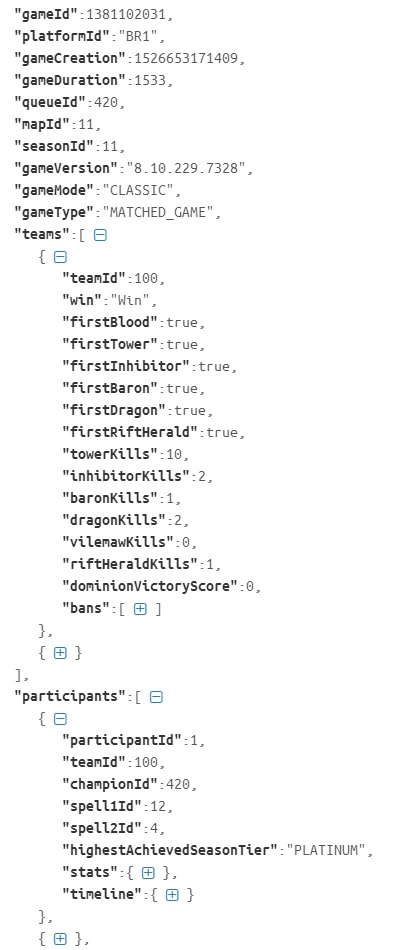
\includegraphics[width=9cm]{imagens/match-v3.jpg}
	\end{center}
	\small{Fonte: Autor.}
	\label{fig:match-v3}
\end{figure}

De todas essas informações retornadas pela função, as que foram armazenadas para o projeto por participante são:

\begin{enumerate}
\item \textit{gameId}. Identificador único da partida;
\item \textit{kills}, \textit{deaths} e \textit{assists}. Informações que falam, respectivamente, quantas vezes esse jogador matou, morreu e participou na morte de outrem;
\item \textit{win}. Se ele ganhou;
\item \textit{championId}. Qual campeão ele escolheu;
\item \textit{lane}. Em qual posição ele tava jogando;
\item \textit{platformId}. Em qual servidor ele jogava;
\item \textit{queueId}. E qual o tipo de partida.
\end{enumerate}

Sabendo qual informação vamos armazenar, ficou escolhido a linguagem \textit{Python} para ser desenvolvido o algoritmo no qual obterá as informações de forma não manual e o sistema de gerenciamento de banco de dados MySQL. Na próxima seção será apresentado sobre banco de dados e na seção \ref{chap:aquisicao} será esclarecido como foram obtidos o \textit{dataset} das partidas. 


\section{Persistência dos dados}
Os dados adquiridos serão armazenados em um banco de dados MySQL, cujo o esquema das tabelas podem ser vistas na Figura \ref{fig:bd}, onde é possível ver quais foram as informações salvas. Com o esquema do banco de dados pronto, já é possível passar para a aquisição dos dados.
\begin{figure}[H]
	\caption{Esquema usado do Banco de Dados.}
	\begin{center}
		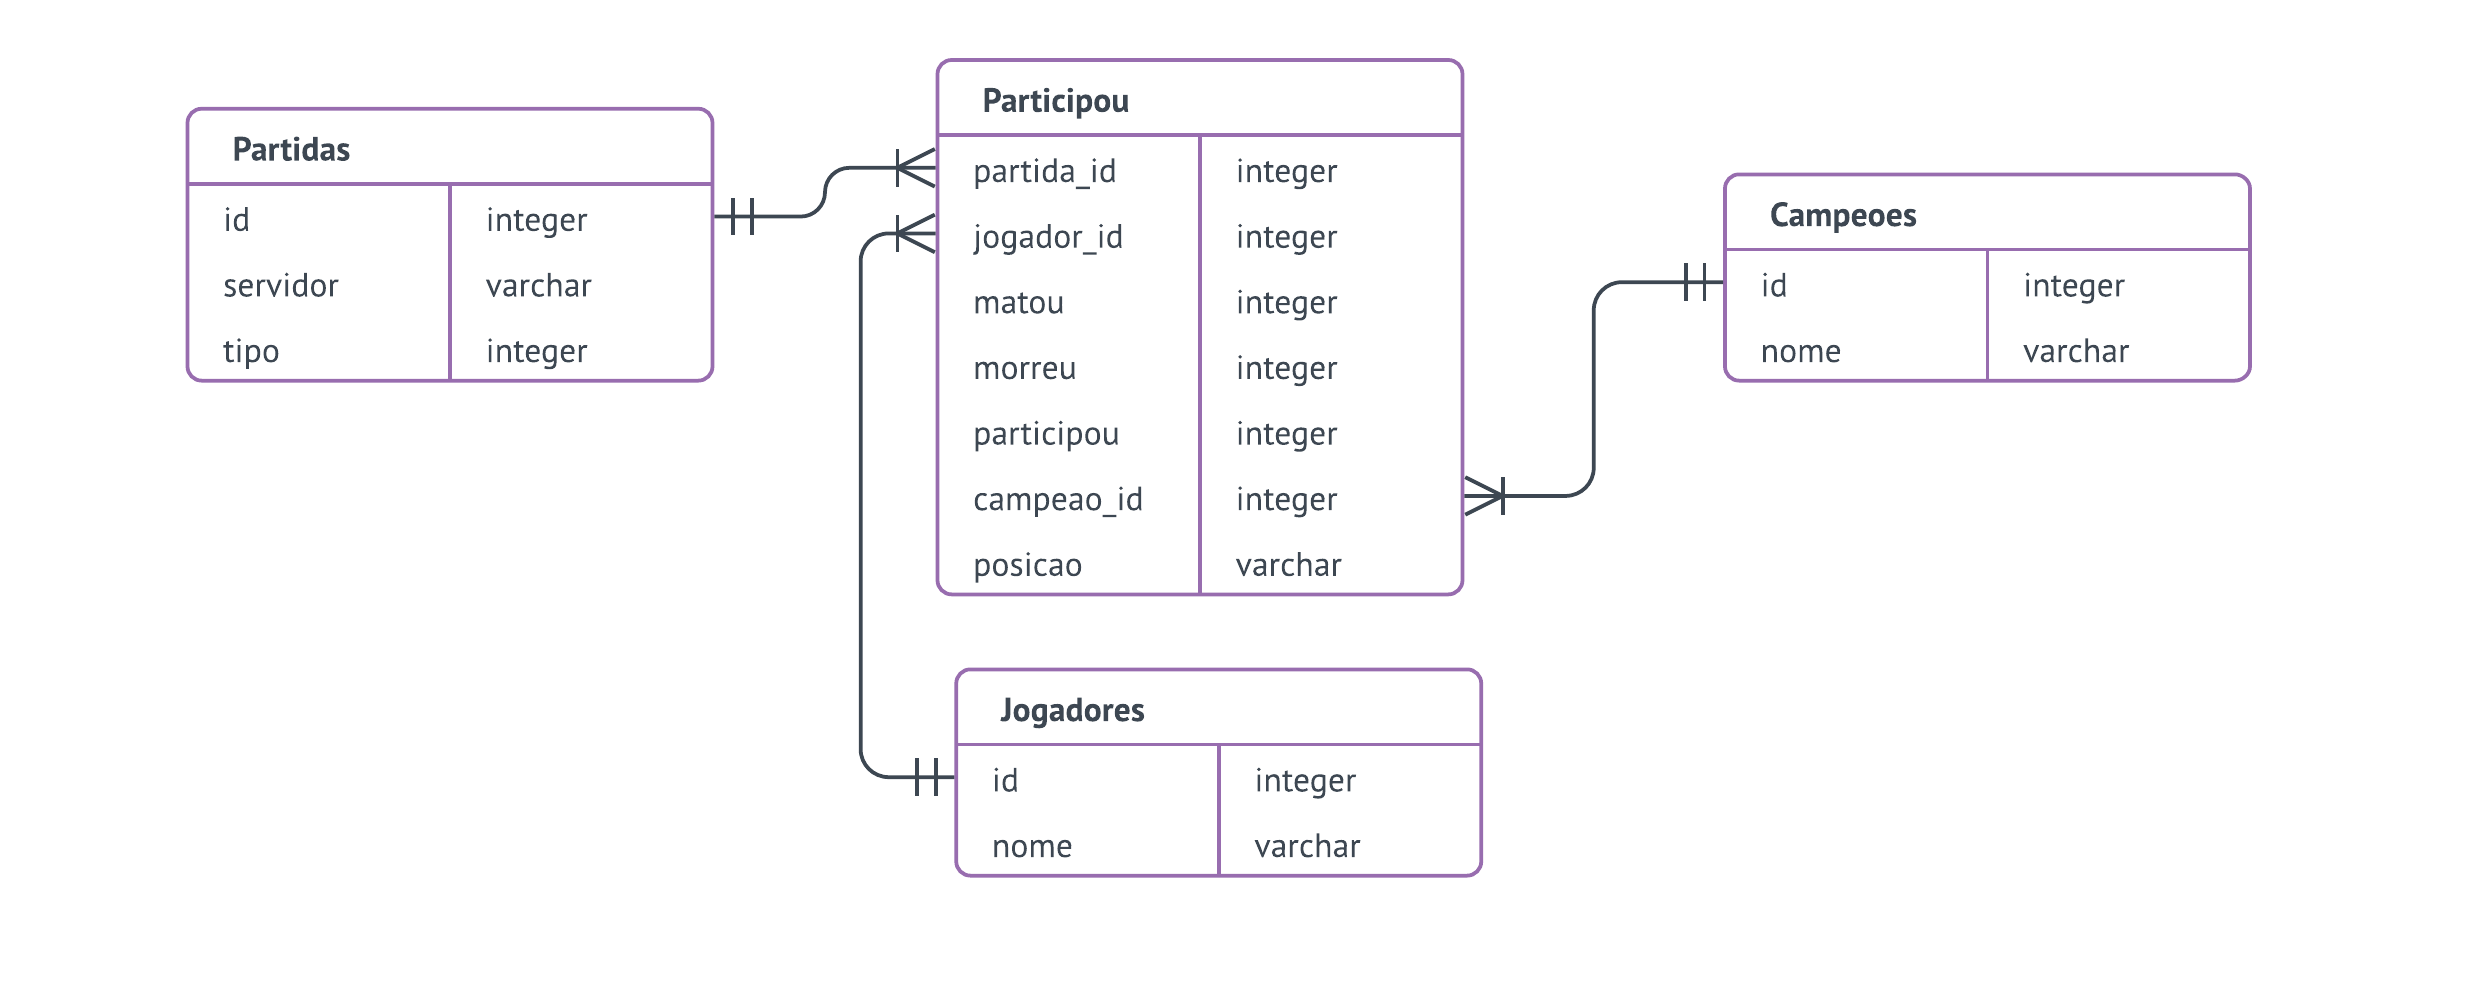
\includegraphics[width=17cm]{imagens/esquema.png}
	\end{center}
	\small{Fonte: Autor.}
	\label{fig:bd}
\end{figure}


\section{Aquisição dos dados}
\label{chap:aquisicao}
A aquisição dos dados será dada à partir de duas fontes: a API da Riot Games; e de um \textit{dataset} público\footnote{https://www.kaggle.com/paololol/league-of-legends-ranked-matches}. Ambos apresentam os mesmos conjuntos de informações em formatos diferentes. Aélm destes, será adquirido outros dados pela API para agilização do trabalho.

A base de dados, na sua versão 9, conta com aproximadamente 183 mil partidas ranqueadas (partidas que, em poucas palavras, servem para classificar as habilidades do jogador) diferentes, dando uma incrementada no banco de dados inicialmente. Estes que precisam ser convertidos para o esquema do banco de dados usados no trabalho.
Em seguida, será usado um algoritmo para a aquisição dos dados de partidas pela API do \textit{League of Legends} em \textit{Python}, que usa a biblioteca \textit{requests} para conseguir acessar a API por URL's, verificando se a partida requisitada existe e se os dados necessários estão completos, salvando no banco de dados apenas as partidas válidas. O pseudo-código se encontra no Algoritmo \ref{alg:main-aqui}.

\
 %Código


\begin{algorithm}[H]
   \SetAlgoLined
     \Inicio{

		i = 1000000000;\tcp*[f]{Esta é a \textit{id} de uma partida aleatória na ultima versão do jogo}
            
		chave = minha chave privada de acesso;
            
        \uSe{Existe arquivo com ultimo partida lido}{
          	i = ultima partida lida;
        }
        \Repita{Até ser pausado}{    
            pedido = requisita URL Da API(i, chave);

            \Se((\tcp*[f]{Se a partida existe}){pedido.status == 200 }{
            	 
            	JSON = carrega JSON Do Pedido(pedido);
                
                \uSe{JSON é válido}{
                	Armazena os dados em um banco de dados;
                }
                
                i = i + 1;

            }
		}
	                
	Salva i no arquivo;
    }
   \label{alg:main-aqui}
   \caption{\textsc{Aquisição dos dados das partidas}}
 \end{algorithm}

\

Decidiu-se usar apenas as partidas ranqueadas 5 contra 5, já que estas são as partidas responsáveis pela classificação dos jogadores dentro dos jogo, e as partidas não ranqueadas são consideradas como amistosas.
Na etapa seguinte são contabilizados quantas vezes cada campeão específico apareceu em uma mesma partida com outro campeão específico, seja no mesmo time ou no time adversário, calculando quantas vitórias em oposição e quantas vitórias em junção.

Com as informações já processadas, foi montado um \textit{web service}, que será explicado na seção \ref{chap:web}, utilizando uma biblioteca chamada D3.js para uma melhor visualização dos dados obtidos , biblioteca essa que será explanado na próxima seção.

\section{Visualização dos dados}
\label{chap:web}

O \textit{web service} será criado utilizando o \textit{framework} Flask, que como \citet[tradução do autor]{flask} diz "Flask é um micro \textit{framework} para Python baseado em Werkzeug, Jinja 2 e em boas intenções.".

Com esse serviço será possível um relatório geral, onde o usuário será capaz de ver a topologia do modelo, vendo quais são os campeões melhores contra os outros e quais são as duplas mais favoráveis, podendo filtrar quais deles podem participar da pesquisa e quais não podem. 
Também será exequível a predição de uma partida, na qual se seleciona os campeões de cada equipe e o sistema tenta antever quem vencerá.



\section{Classificação da topologia}
\label{chap:topo}
Esperando o artigo.

\section{Predição dos dados}
\label{chap:pred}

Para a parte de predição dos dados, serão considerados as conexões e os pesos entre os campeões da partida obtidas através do grafo obtido na Seção \ref{chap:aquisicao}. Os dados de cada partida foram transformados em 3 informações de entrada e a saída:

\begin{itemize}
	\item Sinergia Time 0;
	\item Sinergia Time 1;
	\item Entropia Somada;
	\item Time vencedor.
\end{itemize}

Sendo que as duas primeiras informações se referem a somatória dos pesos da aresta que diz o quão bom os campeões de um time vencem juntos, dados 0 a 1. Para tanto, vamos considerar que\( p_1, p_2, p_3, p_4, p_5 \) são do time 0, \( p_6, p_7, p_8, p_9, p_10 \) do time 1, e \(w(u,v)\) sendo o peso da arestas de porcentagem de partidas ganhas juntas de \(u\) e \(v\), de 0 a 1. Então pode se dizer que: \[ Sinergia Time 0 = \sum_{\overset{1<=i<=5}{i<j<=5}}w(p_i,p_j),\] e, também: \[ Sinergia Time 1 = \sum_{\overset{6<=i<=10}{i<j<=10}}w(p_i,p_j).\]

A entropia somada, foi definida como a soma de quantas partidas um campeão \(c_1\) ganhou de um campeão \(c_2\), sendo que este valor também vai de 0 a 1. A definição matemática pode ser descrita como, sendo \(w_e(c_1,c_2)\) a porcentagem que o \(c_1\) ganhou do \(c_2\) : \[ Entropia Somada = \sum_{\overset{1<=i<=5}{6<=j<=10}}w_e(c_i,c_j)\]

A entropia do time 1 para o time 0 não foi feita, porque a correlação entre as duas entropias seria alta, uma vez que \(w_e(p_i, p_j) = 1 - w_e(p_j, p_i)\) e elas informariam a mesma coisa. Então, por eficiência, e para aumentar a velocidade de treino do modelo, ela foi retirada. O time vencedor apenas diz qual time venceu, informando se foi o time 0 ou o time 1.

Então com esses valores, é criado um classificador KNN, em que, com as três informações de entrada, ele tentará classificar o time vencedor. Os valores que foram armazenados, são separados em dados de treino e de teste, sendo que o teste representam 20\% dos dados totais e todos os dados são re-escalados no intervalo de 0 a 1, para que o KNN possa ser treinado adequadamente.
Com o modelo final treinado e testado, o \textit{webservice} será capaz de comunicar com o KNN para responder às entradas do usuário, indicando um time vencedor.
\